\documentclass[../Main.tex]{subfiles}

\begin{document}
Rotating frames are important examples of non-inertial reference frames.
\section{Newton's Laws in a Rotating Frame}
An inertial frame $S$ has Cartesian axes $\vec{e_1}, \vec{e_2}, \vec{e_3}$. A rotating frame $S'$ has axes $\vec{e_1}', \vec{e_2}', \vec{e_3}'$ that rotate with angular velocity $\omega$ relative to $S$. Therefore, the velocity of one of these axes is $\dvec{e_i}' = \vec{\omega} \times \vec{e_i}'$\par
The position of a particle is:
\begin{equation*}
   \vec{x} = x_i\vec{e_i} = x_i'\vec{e_i}'
\end{equation*}
The velocity of this particle is:
\begin{equation*}
    \dvec{x} = \dot{x}_i \vec{e_i} = \dot{x}_i'\vec{e_i}' + x_i' \vec{\omega} \times \vec{e_i}'
\end{equation*}
We write this equation as:
\begin{equation*}
    \left(\frac{d\vec{x}}{dt}\right)_S = \left(\frac{d\vec{x}}{dt}\right)_{S'} + \vec{\omega} \times \vec{x}
\end{equation*}
Note that here $\left(\frac{d\vec{x}}{dt}\right)_S$ means the derivative of the Cartesian components of the vector in frame $S$. The difference between the two derivatives is the relative velocity of the two frames.\par
The acceleration of the particle is given by:
\begin{equation*}
    \ddvec{x} = \ddot{x_i} \vec{e_i} = \ddot{x}_i' \vec{e_i}' + 2\vec{\omega} \times x_i' \vec{e_i}' + \vec{\omega} \times (\vec{\omega} \times x_i' \vec{e_i}')
\end{equation*}
We can also write:
\begin{equation*}
    \left(\frac{d^2\vec{x}}{dt^2}\right)_S = \left(\frac{d^2\vec{x}}{dt^2}\right)_{S'} + 2\vec{\omega} \times \left(\frac{d\vec{x}}{dt}\right)_{S'} + \dvec{\omega} \times \vec{x} + \vec{\omega} \times \left(\vec{\omega} \times \vec{x}\right)
\end{equation*}
In the inertial frame, Newton's law holds:
\begin{equation*}
    m \left(\frac{d^2\vec{x}}{dt^2}\right)_S = \vec{F}
\end{equation*}
So in the rotating frame:
\begin{equation*}
    m\left(\frac{d^2\vec{x}}{dt^2}\right)_{S'} = \vec{F} - 2m\omega \times \left(\frac{d\vec{x}}{dt}\right)_{S'} - m\dvec{\omega} \times \vec{x} - m\omega \times (\vec{\omega} \times \vec{x})
\end{equation*}
The extra terms on the right-hand side are \underline{fictitious forces}. They all have names:
\begin{itemize}
    \item The term $2 m \omega \times \left(\frac{d\vec{x}}{dt}\right)_{S'}$ is the \underline{Coriolis force}
    \item The term $m \dvec{\omega} \times \vec{x}$ is the \underline{Euler force}
    \item The term $m \vec{\omega} \times (\vec{\omega} \times \vec{x})$ is the \underline{centrifugal force}.
\end{itemize}
\begin{remark}
    We will often consider the Earth as a rotating reference frame. For this case, $\vec{\omega}$ is approximately constant, so the Euler force can be disregarded.
\end{remark}
\section{The Centrifugal Force}
The centrifugal force is:
\begin{equation}
    \vec{F_{cen}} = -m \vec{\omega} \times (\vec{\omega} \times \vec{x})
    \label{eqnCentrifugal}
\end{equation}
This is illustrated in figure~\ref{figCentrifugal}.
\begin{figure}[ht]
    \centering
    See the diagram Centrifugal force. %TODO: Tikz this.
    \caption{Diagram of the direction of the centrifugal force}
    \label{figCentrifugal}
\end{figure}
The centrifugal force points away from the axis of rotation. It has magnitude:
\begin{equation*}
    |\vec{F_{cen}}| = m\omega^2 r \cos{\theta} = m\omega^2d
\end{equation*}
Where the quantities $r$, $d$, $\theta$ are as in figure~\ref{figCentrifugal}.\par
The centrifugal force is conservative:
\begin{align*}
    \vec{F_{cen}} &= -\nabla\left(-\frac{m}{2}|\vec{\omega} \times \vec{x}|^2\right) \\
    &= -\nabla\left(-\frac{m}{2}\omega^2r^2\cos^2\theta\right) \\
    &= -\nabla\left(-\frac{m}{2}\omega^2d^2\theta\right)
\end{align*}
The potential energy is decreased by the particle moving away from its axis of rotation.
\begin{figure}[ht]
    \centering
    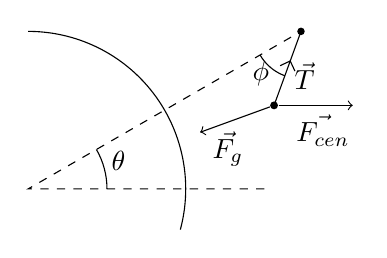
\begin{tikzpicture}[scale=2]
        \tikzset{
            patharrow/.pic={
                \draw (-0.1, -0.1) -- (0, 0) -- (-0.1, 0.1);
            }
        }
        \draw (-15:1) arc[start angle=-15, end angle=90, radius=1];
        \draw (0:0.5) arc[start angle=0, end angle=30, radius=0.5]
            node[anchor=west, pos=0.7] {$\theta$};

        \draw[dashed] (0:1.5) -- (0:0) -- (30:2);
        \draw[fill] (30:2) circle[radius=0.2mm];

        \draw (30:2) -- ++(250:0.5)
            pic[pos=0.4, rotate=70] {patharrow}
            node[pos=0.6, anchor=west] {$\vec{T}$}
            node[circle, fill, minimum size=1mm, inner sep=0] (A) {};
        \draw (30:1.7) arc[start angle=210, end angle=250, radius=0.3]
            node[anchor=east, pos=0.8] {$\phi$};

        \draw[->] (A) -- +(200:0.5)
            node[pos=0.6, anchor=north] {$\vec{F_g}$};

        \draw[->] (A) -- +(0:0.5)
            node[pos=0.6, anchor=north] {$\vec{F_{cen}}$};
    \end{tikzpicture}
    \caption{Diagram of example~\ref{exHangingString}: a hanging string}
    \label{figHangingString}
\end{figure}
\begin{example}[Hanging string]
    Consider figure~\ref{figHangingString}.
    The forces are:
    \begin{equation*}
        \vec{F_g} = -mg\uvec{r}
    \end{equation*}
    \begin{align*}
        \vec{F_{cen}} &=-m \vec{\omega} \times (\vec{\omega} \times \vec{x}) \\
        &= m\omega^2 r\cos{\theta} \left(\cos{\theta}\uvec{r} - \sin{\theta} \uvec{\theta}\right)
    \end{align*}
    If the string makes an angle $\phi$ with the radial direction,
    \begin{equation*}
        \vec{T} = T\cos{\phi}\uvec{r} + T\sin{\phi}\uvec{\theta}
    \end{equation*}
    In equilibrium, the forces must balance:
    \begin{align*}
        -mg + m\omega^2 r \cos^2\theta + T\cos{\phi} &= 0 \\
        -m\omega^2 r \cos{\theta}\sin{\theta} + T\sin{\phi} &= 0 \\
    \end{align*}
    Solving for $T$ and $\phi$:
    \begin{equation*}
        \tan{\phi} = \frac{\omega^2 r cos{\theta} \sin{\theta}}{g - \omega^2 r \cos^2{\theta}}
    \end{equation*}
    \label{exHangingString}
\end{example}
\section{Coriolis Force}
The Coriolis force is given by:
\begin{equation}
    \vec{F_{cor}} = -2m\vec{\omega} \times \vec{v}
    \label{eqnCoriolis}
\end{equation}
The force is dependent on velocity but independent of position. It has the same form as the Lorentz force, with $\vec{B} \to \vec{\omega}$, so moving particles will turn in circles.
\subsection{Examples of the Coriolis Force}
\begin{example}[Hurricanes]
    The Coriolis force is responsible for the formation of hurricanes.\par
    Hurricanes are formed by a low-pressure region of air. Where winds blow inward toward this low-pressure zone, the Coriolis force causes the air particles to rotate and causes swirling winds around the original low-pressure zone. This effect is less near the equator, where the Coriolis force acts normal to the surface of the earth, but does not overcome gravity.
\end{example}
\begin{figure}[ht]
    \centering
    See the diagram Ball from Tower %TODO: Tikz this
    
    \caption{Diagram of a ball falling from a tower, for example~\ref{exBallFromTower}}
    \label{figBallFromTower}
\end{figure}
\begin{example}[Dropping a ball from a tower at the equator]
    We can guess the answer from conservation of angular momentum: initially the ball has angular momentum $l = (R + h)^2 \omega$, but as the ball falls the distance to the axis of rotation decreases, so its angular speed must increase. At the foot of the tower, $l = R^2 \omega'$ so $\omega' > \omega$. This effect is due to the Coriolis force.\par
    In a rotating frame we consider Newton's Law:
    \begin{equation}
        \ddvec{x} = \vec{g} - 2\vec{\omega} \times \dvec{x}
        \label{eqnBallFromTowerMotion}
    \end{equation}
    Note that we neglect the centrifugal force, since it is parallel to $\vec{g}$ and is much weaker than it.\par
    Note that equation~\ref{eqnBallFromTowerMotion} has no term in $\vec{x}$, so integrating once:
    \begin{equation*}
        \dvec{x} = \vec{g}t - 2\vec{\omega} \times \left(\vec{x} - \vec{x_0}\right)
    \end{equation*}
    Here $\vec{x_0}$ is the constant of integration.\par
    Substituting this back into equation~\ref{eqnBallFromTowerMotion}:
    \begin{align*}
        \ddvec{x} &= \vec{g} - 2\vec{\omega} \times \vec{g}t + 4 \omega \times \left(\omega \times \left(\vec{x} - \vec{x_0}\right)\right) \\
        &= \vec{g} - 2\vec{\omega} \times \vec{g}t \text{ by neglecting forces parallel to } \vec{g}
    \end{align*}
    Then integrating this (assuming the ball was dropped from rest):
    \begin{equation*}
        \vec{x} = \vec{x_0} + \frac{1}{2} \vec{g} t^2 -\frac{1}{3} \vec{\omega} \times \vec{g} t^3
    \end{equation*}
    Now consider a basis: $\vec{e_1}$ in the north direction, $\vec{e_2}$ in the west direction and $\vec{e_3}$ in the upward direction. Here $\vec{\omega} = \omega \vec{e_1}$, $\vec{g} = -g\vec{e_3}$ and $\vec{x_0} = (R + h) \vec{e_3}$. Therefore $\vec{x}$ is:
    \begin{equation*}
        \vec{x} =
        \begin{pmatrix}
            0 \\
            -\frac{1}{3}gt^3 \\
            R + h - \frac{1}{2}gt^2
        \end{pmatrix}
    \end{equation*}
    And so $\vec{e_2}$ is negative when the ball hits the ground. That is, the ball hits the ground east of the tower.
    \label{exBallFromTower}
\end{example}
\subsection{Extended Example: Foucault's Pendulum}
Consider a pendulum at the North Pole. As the Earth rotates under the pendulum, from the point of view of an observer on the Earth, the pendulum will appear to rotate. At a general angle latitude $\theta$, we consider the motion of the pendulum in the rotating reference frame. Consider again a basis such that $\vec{e_1}$ is north, $\vec{e_2}$ is west, and $\vec{e_3}$ is north.
We choose:
\begin{align*}
    \vec{x} &= (x, y, z)^T \\
    \vec{g} &= (0, 0, -g)^T \\
    \vec{\omega} &= (\omega \cos{\theta}, 0, \omega \sin{\theta})^T
\end{align*}
Consider a pendulum of length $l$ in figure~\ref{figFoucaultPendulum}.
\begin{figure}[ht]
    \centering
    \tdplotsetmaincoords{70}{20}
    \begin{tikzpicture}[tdplot_main_coords, scale=2]
        \draw[->] (0, 0, 0) -- (1, 0, 0) node[right] {$\vec{e_1}$};
        \draw[->] (0, 0, 0) -- (0, 2, 0) node[right] {$\vec{e_2}$};
        \draw[->] (0, 0, 0) -- (0, 0, 2) node[above] {$\vec{e_3}$};

        \draw[Bar-Bar] (-0.2, 0, 0) -- (-0.2, 0, 1.4) node[pos=0.5, left] {$l$};
        \fill (0, 0, 1.4) circle[radius=0.2mm];
        \fill (0.4, 0.6, 0.2) circle[radius=0.2mm];

        \draw (0.4, 0.6, 0.2) -- (0, 0, 1.4)
            node[pos=0.7, anchor=west] {$\vec{T}$};
        \draw (0.18,0.26,0.72) -- (0.2, 0.3,0.8) -- (0.28,0.38,0.76);

        \draw[densely dotted] (0.4, 0.6, 0.2)
            -- (0.4, 0.6, 0) -- (0.4, 0, 0);
        \draw[densely dotted] (0.4, 0.6, 0) -- (0, 0.6, 0);
        \draw (0.4, 0, 0) -- (0.4, -0.1, 0) node[below] {$x$};
        \draw (0, 0.6, 0) -- (-0.1, 0.6, 0) node[above] {$y$};
        \draw[Bar-Bar] (0.5, 0.6, 0) -- (0.5, 0.6, 0.2)
            node[pos=0.5, right] {$z$};
    \end{tikzpicture}
    \caption{Diagram of Foucault's Pendulum}
    \label{figFoucaultPendulum}
\end{figure}
Then we can write down the tension:
\begin{equation*}
    \vec{T} = (-T\frac{x}{l}, -T\frac{y}{l}, T\frac{l - z}{l})
\end{equation*}
The string has a fixed length so we have the constraint that $x^2 + y^2 + (l - z)^2 = l^2$. Alternatively, $|\vec{T}| = T$.
The equation of motion is:
\begin{equation}
    m\ddvec{x} = \vec{T} + m\vec{g} - 2m\vec{\omega} \times \dvec{x}
    \label{eqnFoucaultMotion}
\end{equation}
We have 3 differential equations and one constraint, so we can work out the 4 quantities: $|\vec{T}, x, y, z$.\par
The solution is by initially eliminating $z$, then solving for $T$. This leaves two coupled differential equations for $x$ and $y$, solved by considering $x + iy$.\par
The solution that is eventually reached is:
\begin{equation}
    x + iy = e^{-i\omega t \sin{\theta}} \left[a \cos{\left(\sqrt{\frac{g}{l} t}\right)} + b \sin{\left(\sqrt{\frac{g}{l} t}\right)}\right]
    \label{eqnFoucaultSolution}
\end{equation}
Here $a$ and $b$ are complex constants that are determined by initial conditions. This shows that the pendulum follows an ellipse in the $x-y$ plane that slowly rotates. We can determine exactly the speed of rotation:
\begin{equation*}
    T = \frac{24\text{ hours}}{\sin{\theta}}
\end{equation*}
In France, where the original Foucault Pendulum is, the period is 32 hours. On the North Pole, it is 24 hours and at the equator the effect is not seen.
\end{document}